\tikzset{%
  >=latex
}
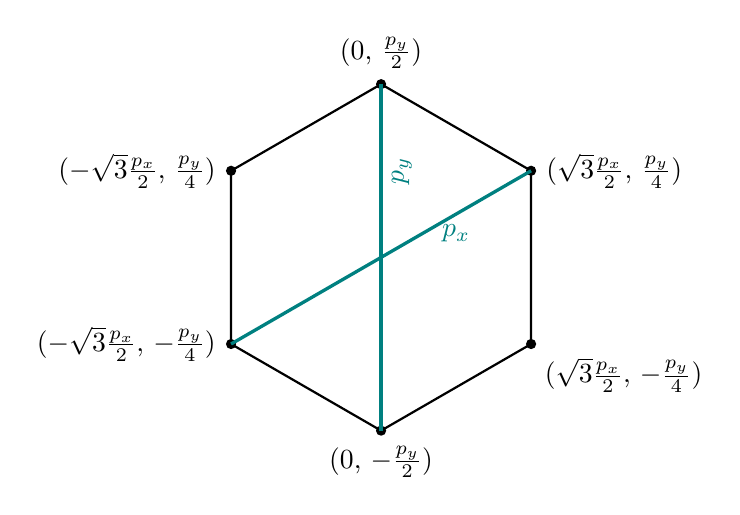
\begin{tikzpicture}[thick]
     \newdimen\R
     \R=2.2cm
     \draw (330:\R) \foreach \x in {30,90,...,330} {  -- (\x:\R) };
     \foreach \x/\l/\p in
       { 30/{($\sqrt{3} \frac{p_x}{2}$, $\frac{p_y}{4}$)}/right,
        90/{($0$, $\frac{p_y}{2}$)}/above,
        150/{($-\sqrt{3} \frac{p_x}{2}$, $\frac{p_y}{4}$)}/left,
        210/{($-\sqrt{3} \frac{p_x}{2}$, $-\frac{p_y}{4}$)}/left,
        270/{($0$, $-\frac{p_y}{2}$)}/below,
        330/{($\sqrt{3} \frac{p_x}{2}$, $-\frac{p_y}{4}$)}/below right
       }
       \node[inner sep=1pt,circle,draw,fill,label={\p:\l}] at (\x:\R) {};

       \draw[very thick, teal] (30:\R) -- (210:\R) node[near start, below] {$p_x$};

       \draw[very thick, teal] (270:\R) -- (90:\R) node[sloped, near end, below] {$p_y$};

\end{tikzpicture}
